\documentclass[lettersize,journal]{IEEEtran}
\usepackage{algorithmic}
\usepackage{algorithm}
\usepackage{amsmath,amsfonts}
\usepackage{array}
\usepackage{arydshln} % for horizontal dashed lines in table
\usepackage{balance}
\usepackage{cite}
\usepackage{gensymb} % for degrees symbol
\usepackage{graphicx}
\usepackage{stfloats}
\usepackage[caption=false,font=normalsize,labelfont=sf,textfont=sf]{subfig}
\usepackage{tabularx}
\usepackage{textcomp}
\usepackage{url}
\usepackage{verbatim}
\usepackage{xcolor}

\hyphenation{op-tical net-works semi-conduc-tor IEEE-Xplore}

\begin{document}

\title{Modelling of Diffuse Scattering Effects for Outdoor Ray Tracing}
\author{Andrew Whelan, \emph{Dublin City University}^*\thanks{*Thanks to Prof. Conor Brennan - who provided very useful guidance.}}

% The paper headers
\markboth{MEng in Electronic \& Computer Engineering}%
{Shell \MakeLowercase{\textit{et al.}}: Modelling of Diffuse Scattering Effects for Outdoor Ray Tracing - Literature Review}

\maketitle

\begin{abstract}
Geometrical Optics (GO) models electromagnetic (EM) propagation as rays which interact with surfaces (or media-boundaries) by splitting into one reflected and one absorbed ray, the direction and amplitude of which are determined simply by angle of incidence and refractive indices. Such ``specular reflection'' (SR) lends itself to a ray tracing (RT) simulation. SR is, however, only adequate under restrictive assumptions, which are becoming less tenable with increasing EM-wave frequencies, more complex surfaces, materials, and environments. Such complexities are typical for a modern urban scenario and for new wireless technologies, where ``diffuse scattering'' (DS) is the norm. DS is the phenomenon whereby reflected radiation is scattered among many directions (and not just the specular one). In this paper we evaluate work done by various authors on  DS models and conclude that, for outdoor RT purposes, the most promising avenue of research is heuristic (parametric) modelling, specifically in dynamic environments, and that there are is also significant opportunity for improving the flexibility of ray-tracing software.
\end{abstract}

\begin{IEEEkeywords}
Diffuse Scattering, Diffuse Reflection, Channel Model, Ray Tracing, Ray Shooting.
\end{IEEEkeywords}

\section{Introduction}
\IEEEPARstart{F}{or} RT purposes, the theory of GO can be summarised by (see Fig. \ref{diag:GOSetup}):

\begin{subequations}\label{eq:GO}
	\begin{align}
		\left( \theta_R, \theta_T \right) &= \left( \theta_I,  \sin^{-1} \left( \frac{n_I}{n_T}\sin\theta_I \right) \right) \label{eq:directionalityGO} \\
		r =(r_{\parallel}, r_{\perp}) &= \left( \frac{\tan(\theta_I - \theta_T)}{\tan(\theta_I+\theta_T)}, -\frac{\sin(\theta_I - \theta_T)}{\sin(\theta_I+\theta_T)} \right), \label{eq:fresnelR} \\
		t = (t_{\parallel},t_{\perp}) &= \left( \frac{n_I}{n_T}(r_{\parallel} + 1), r_{\perp} + 1, \right). \label{eq:fresnelT}
	\end{align}
\end{subequations}
\begin{figure}[t]
	\centering
	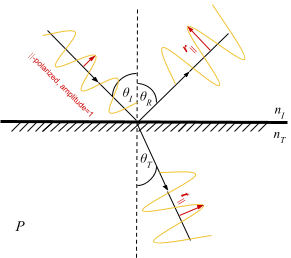
\includegraphics[width=2.8in]{GO Setup}
	\captionsetup{singlelinecheck=off}
		\caption[]{GO setup. The incoming and reflected rays determine a plane of incidence $P$. Knowledge of (i) refractive indices ($n_I$,$n_T$), (ii) $\theta_I$, (iii) amplitude and phase of incident ray, and (iv) polarization, is enough to determine the outgoing radiation. The example above assumes the incident radiation has zero-phase, unit-amplitude, and is polarized parallel to $P$. The subscripts $\parallel$ and $\perp$ denote the components of the field parallel and perpendicular to $P$.
	} 
	\label{diag:GOSetup}
\end{figure}
Equations \eqref{eq:directionalityGO} give directional information for the reflected and transmitted portions, whereas \eqref{eq:fresnelR} and \eqref{eq:fresnelT} give the amplitude, phase and polarization of the EM-field.

This formulation predates Maxwell's theory, and is limited in several respects. Mainly, EM-radiation can diffract and undergo DS due to the relationship between the wavelength of the radiation and the ``wavelength'' of the surface (classically, the roughness, but also molecular anomalies of surface materials). While the diffraction can be treated via the ``Uniform-Theory of Diffraction'', the formulation of a practical DS model, especially for RT-software, has been tricky, and only treated adequately in the last 20 or so years. 

The beginnings of modelling DS is with J.H Lambert.  Whilst SR is one extreme for an ideally flat, mirror-like surface, Lambert considered the other extreme  - an ideally rough ``matte-like'' surface. The idea is that such a surface is perceived as having constant brightness as the observer's angle changes. Analyzing this gives us the concept of a Lambertian-pattern - where the scattering pattern looks like:
\begin{equation}
E_S = E_0\sqrt{\cos(\theta_S)}, \label{eq:Lambertian}
\end{equation}
where $\theta_S$ is the scattering angle, $E_S$ is the amplitude,and $E_0$ is the maximum amplitude in the direction of the surface normal. Equation \eqref{eq:Lambertian} is often taken as a hypothesized pattern of DS. An example can be seen in red in Fig. \ref{diag:scattering}.


However, since the derivation of the pattern in equation \eqref{eq:Lambertian} also predates Maxwell, such parametric models have been labelled as ``heuristic'', resulting in two types of theories - ``heuristic'' and ``physical''.

The aim of this project is to identify areas of improvement broadly for modelling such phenomena. So, in evaluating existing models, the following criteria are considered:
\begin{itemize}
\item What is the scattering hypothesis (analogue of \eqref{eq:Lambertian}) ?
\item How are the model-parameters estimated?
\item How is the model integrated with existing RT software?
\item How(-much) was the model validated?
\end{itemize}

\pagebreak

\section{Review and Analysis of Prior Work}
\begin{figure}[b]
	\centering
	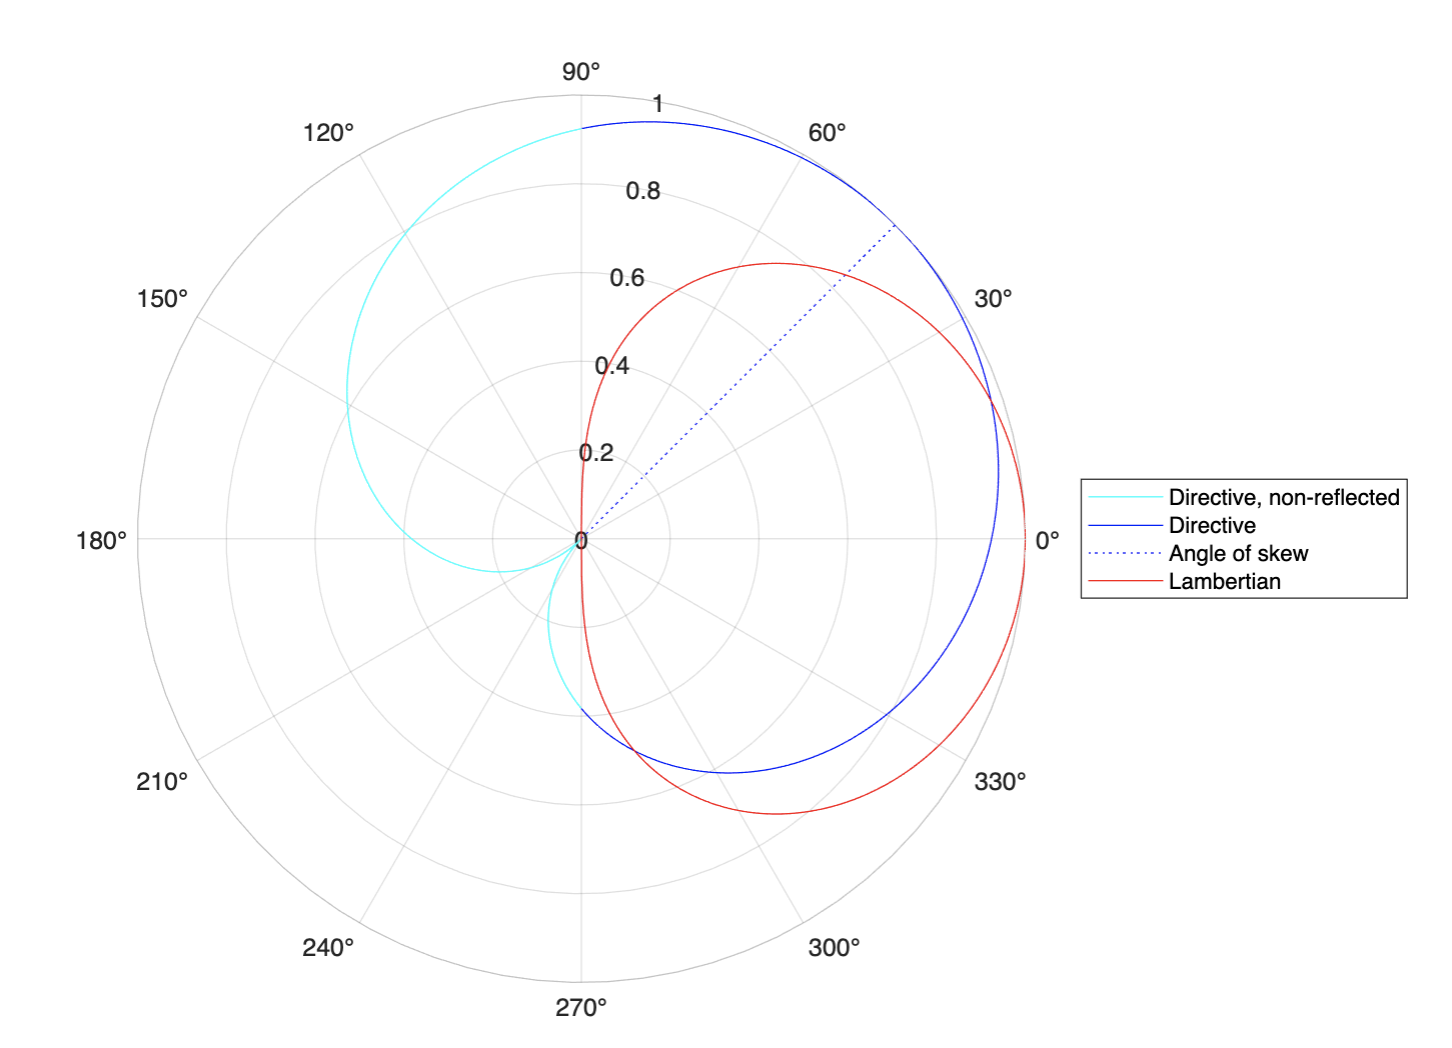
\includegraphics[width=3.1in]{ScatteringPatterns}
	\captionsetup{singlelinecheck=off}
		\caption[]{Scattering patterns for models in sections \ref{lambModel} and \ref{directiveModel}. The ``angle of skew'' is the $\phi_S$ referred to in Fig. \ref{diag:BeckmannAngles} and in equation \eqref{eq:directiveModel}. Here $\phi_S = 45 \degree$. }
	\label{diag:scattering}
\end{figure}

The survey conducted filtered papers based on keywords ``diffuse ray tracing''. 451 papers were found in the literature, to which the following filters were applied:
\begin{enumerate}
    \item Title - many of the papers were not of relevance to the topic, and additionally some focussed on applications of models, e.g. graphics ;
    \item Abstract - once the above filters were applied, the abstracts were read with similar goals in mind ;
    \item Indoor-only models removed.
\end{enumerate}
This gave a resulting 52 papers. Citation numbers were then used as a rough guide on priority.

In what follows will be subsections outlining the type of model. For each of these there are the following important validation-measures:
\begin{enumerate}
	\item power distributions ($E_S$ vs. some variable):
	\begin{enumerate}
		\item Power-Spatial-Profile (PSP) - vs. wall position $x$,
		\item Power-Delay-Profile (PDP) - vs. time-delay $t$,
		\item Power-Angle-Profile (PAP) - vs. $\theta_S$,
	\end{enumerate}
	\item channel-dispersion measures, such as delay-spread, and
	\item computational complexity.
\end{enumerate}

\subsection{``Heuristic'' Effective-Roughness (ER) Models} \label{heuristicModels}
All ER-models considered in the literature have an important ``peak''-intensity $E_0$ associated with the scattering pattern. What's important is that $E_0$ can be derived by equating the power flowing through the diffuse radiation cone (integral expression), with $S^2$ (ratio of the scattered power to the incoming power) times the power flowing through the specular radiation cone ($E^2r_i^2dW$). For instance, for the pattern in equation \eqref{eq:Lambertian}, $E_0$ can be calculated \cite{ref:degliSecond} as
\begin{equation}
E_{0}^2 = k_I \frac{ \ S^2 \cos(\theta_I)}{l_T l_R} dW. \label{eq:LambertianPower}
\end{equation}
where $k_I$ is a constant depending on incoming wave amplitude, $(l_R, l_T)$ are distances from antennas to wall PoC, and $dW$ is a surface element.

The important parameter in the ER model is $S$. Determining a sensible value for a model in terms of other known parameters is crucial, as $S$ is to account for surface and material irregularities. In \cite{ref:degliThird} $S$ is interpreted by assuming energy-conservation and independence of transmitted-energy and wall-geometry:
\begin{equation}
S \approx \Gamma \sqrt{1- R^2}.
\end{equation}
This gives a good formula for estimating $S$ in terms of $R$ which is the reduction factor to the reflected power (a correction-factor to $\Gamma$ for DS). $R$ itself is expressible \cite{ref:degliSecond} in terms of the standard deviation of surface roughness $\sigma_h$.

\subsubsection{Lambertian Model} \label{lambModel}
This model is described in equations \eqref{eq:Lambertian} and \eqref{eq:LambertianPower}.  
Scattering contribution for a single bounce can be derived \cite{ref:degliSecond,ref:degliThird} for the following measures via equations \eqref{eq:Lambertian} and  \eqref{eq:LambertianPower}:
In \cite{ref:degliSecond} this model was shown to give modest improvements in predicting the PSP when adding a single bounce contribution, once the model parameters are tuned to experimental data.
\subsubsection{Directive-Model} \label{directiveModel}
As outlined in \cite{ref:degliThird} the scattering in this model is centred on the specular direction instead of the surface-normal and is given the following form :
\begin{equation}
	E_s = E_0 \left(\frac{1+ \cos(\theta_S-\phi_S)}{2} \right)^{\frac{\alpha}{2}}, \label{eq:directiveModel}
\end{equation}
where $\phi_S$ is shown in Fig. \ref{diag:BeckmannAngles}, and $\alpha \in \mathbb{Z}^{+}$ is a parameter inversely related to the width of the scattering pattern.
An analogue of \eqref{eq:LambertianPower} is obtained and PAPs in various settings are validated against experimental data. By tuning the directivity parameter $\alpha$ according to $S$ it was found that this model makes an improvement on PAPs when compared to the Lambertian model. Authors in \cite{ref:directiveRepl} replicate these findings in an outdoor scenario in addition to re-validating that the delay-spread isn't improved by much.

\subsubsection{Double-Lobe} \label{doubleLobe}
This is just a directive-model with the following characteristics:
\begin{itemize}
    \item A second directive component in the incident direction - with an accompanying second independent directivity parameter; and
    \item An interpolation parameter $\Lambda$ between the power of each component, with $\Lambda=1$ degenerating into the previous model.
\end{itemize}

Unfortunately, the paper introducing this model \cite{ref:degliThird} validated this against a scenario in which minimal back-scattering is to be expected, and the directive model was evaluated as better in those scenarios.

\subsection{``Physical'' Beckmann-Kirchoff (BK) Models} \label{bkModels}
\begin{figure}[t]
\centering
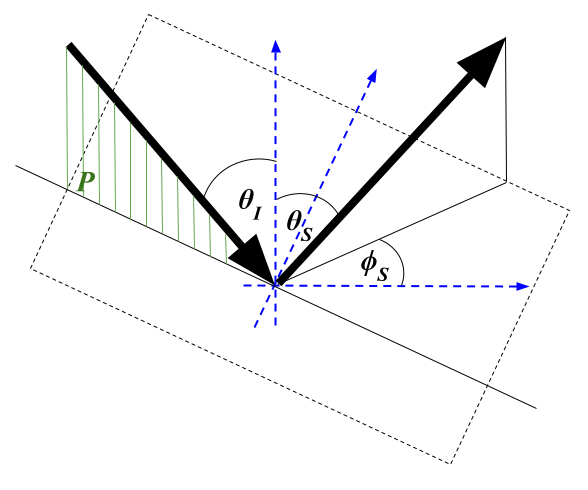
\includegraphics[width=2.5in]{Beckmann Angles}
\captionsetup{singlelinecheck=off}
\caption[]{Scattering geometry setup for the BK and directive-ER models. Diagram is taken from \cite{ref:BK1} and repurposed to correspond with Fig. \ref{diag:GOSetup}. Note that, when $\phi_S=0$ the diagrams are in the same plane, and the diagrams correspond completely when we further impose $\theta_S=\theta_I$.} 
\label{diag:BeckmannAngles}
\end{figure}
These are described in \cite{ref:BK1,ref:BK2}. Essentially, the ratio 
\begin{equation*}
S_R := \frac{E_S}{E_R}
\end{equation*}
is treated statistically, and its mean value is derived as a function of the following deterministic variables:
\begin{itemize}
    \item $\theta_I, \theta_S$,
    \item $\phi_S$, the scattering angle away from wall (see Fig. \ref{diag:BeckmannAngles}),
    \item $\lambda$, the EM-wavelength ,
    \item $dW$, the surface element,
\end{itemize}
and the following statistical parameters:
\begin{itemize}
    \item $\sigma_h$, the standard deviation surface height, and
    \item $l_{\text{corr}}$, the ``correlation-length'', which is somewhat akin to the average spacing of bumps.
\end{itemize}

In \cite{ref:BK2, ref:BK3}, the model is validated (PAP + transfer function) for THz frequencies and a plaster wall. 

The main model limitations are outlined by the ER-model originators in \cite{ref:reciprocalHeur}:
\begin{itemize}
    \item The correlation function used to compute $l_{\text{corr}}$ along with the distribution used to compute $\sigma_h$ are assumed to be Gaussian ;
    \item It requires a knowledge of  $l_{\text{corr}}$ and $\sigma_h$ for a material ;
    \item It ignores internal surface material irregularities ;
    \item It requires weak surface-irregularity: $\lambda \ll l_{\text{corr}} \ll dW$.
\end{itemize}

\subsection{Complications in Outdoor Modelling}
The literature discussed so far has been mainly in the context of a small setup environment (``single-bounce''), where: \begin{itemize}
    \item the line-of-sight (LoS) and first-bounce components of the radiation are assumed to constitute the vast bulk of the received signal ; and
    \item the environment is considered static.
\end{itemize} However, in an outdoor scenario, these are rarely the case. One needs to consider how to incorporate the static models described in sections \ref{heuristicModels} and \ref{bkModels} into an estimation of higher-order non-LoS (NLoS) components, and also how to account for a dynamic environment.

\subsubsection{RT Algorithm}
The question of a RT technique is discussed in \cite{ref:RTComparison}. The authors outline two broad categories. The first is ``ray-shooting'' - where we simulate rays for discrete angles via equations \eqref{eq:directionalityGO} and set an $\epsilon$-radius of tolerance for ``received''. The second is the ``image-method'' in which reflected paths are calculated geometrically. The idea in a simple case (when the ray connecting the virtual Tx with the Rx intersects the wall) is that we construct a virtual Tx by reflecting in the plane of interest and connect this via a line to the Rx to determine the correct point of reflection. Since it's a little cumbersome to explicitly detail the algorithm, an indicative sketch is given in Fig. \ref{diag:imageMethod}.

\begin{figure}[b]
\centering
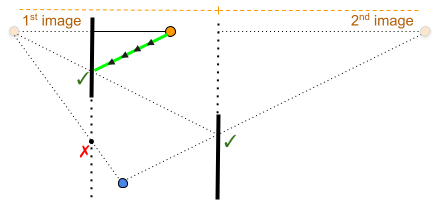
\includegraphics[width=3.5in]{Image method}
\captionsetup{singlelinecheck=off}
	\caption[]{Image-RT method. The Tx is shown in orange and the Rx in blue. On a first iteration it fails, but reflecting the 1st image in the second wall (one to the right) and connecting the second virtual Tx to the Rx, then tracing back, results in a valid path.}
\label{diag:imageMethod}
\end{figure}

One approach to tackling integrating the DS component into an RT simulator is, roughly, as follows \cite{ref:fieldPrediction}. The idea is to build a visibility tree for  ``nodes'' - parts of building walls (for SR and DS), wedges (for diffraction) and the Rx/Tx :

\begin{enumerate}
\item Starting at the Tx, determine the first level of visible nodes according to $N_r$ the number of desired launched rays. In the visibility-tree, draw a branch from the Tx node to each of these, ``terminating'' the node if it's the Rx;
\item For each node in the first layer, for instance a wall, and for each type of interaction, say DS, determine the next layer of nodes visible. Label the new branches with possible interaction types. Again, terminate a node if it's the Rx;
\item Do this recursively until we end up at the maximum number of interactions $N_{ev}$; 
\item Finally, backtrace the power-loss contributions from the leaf nodes along each branch. In the case of DS, the contribution can be done by integrating a formula akin to equation \eqref{eq:Lambertian}+\eqref{eq:LambertianPower}.
\end{enumerate}

%\begin{figure}[t]
%\centering
%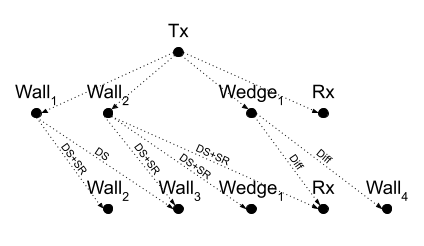
\includegraphics[width=2.5in]{Visibility Tree}
%\captionsetup{singlelinecheck=off}
%\caption[]{Example visibility-tree for $N_{ev}=1$ (i.e. single-bounce). Note that $\text{Wall}_3$ is not visible from $\text{Wall}_1$ via SR. Diagram is repurposed from \cite{ref:fieldPrediction}.} 
%\label{diag:visTree}
%\end{figure}

\subsubsection{Dynamic Environments} \label{dynSection}
There is much to say on this topic. An outdoor environment can change EM scattering significantly as a result of a moving Rx/Tx, due to traffic, moving bridges, etc. The following questions need to be answered:
\begin{itemize}
    \item How long does a given RT simulation take to run?
    \item How frequently \emph{should} it be run in order to be accurate?
    \item Can we make any assumptions on movements that would temporarily obviate the need for resimulation?
\end{itemize}
In \cite{ref:dynamicRTPaper}, the last question is discussed. A database of the initial 3D-environment with moving objects (antennas + cars) and their respective initial velocities and accelerations is assumed. Then, the initial ``ray-chains'' (aka ``multipaths'') are computed via the image-method (as described above and in Fig. \ref{diag:imageMethod}). Under an assumption of a known non-zero multipath lifetime ($T_{\text{life}}$), the instantaneous velocities of the multipath reflection points are then derived. PDPs are compared to regular approaches and can be made to be accurate on calibrating $T_{\text{life}}$, with a computational speedup factor of $\sim$ 50 compared to the regular image-method.

\pagebreak

\section{Relation of Prior Work to the Project Problem}

\begin{figure}[!htb]
\centering
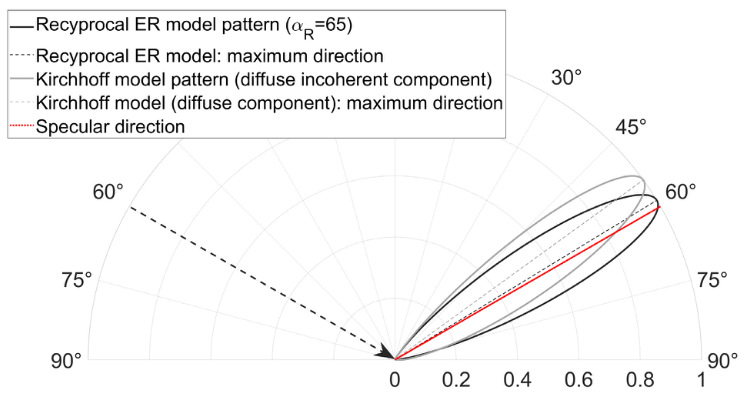
\includegraphics[width=2.8in]{parametricForm}
\captionsetup{singlelinecheck=off}
	\caption[]{The scattering pattern for an ER (see section \ref{heuristicModels}) vs. a BK (see section \ref{bkModels}) model (diagram taken from \cite{ref:reciprocalHeur}). Note the similarity under a rotation.}
\label{diag:parametricForm}
\end{figure}

As per the previous section, there are several avenues of research available in DS-modelling in an outdoor environment.

For instance, one could take a look at validating the model of section \ref{doubleLobe} in better-suited conditions.

For future applications it's necessary to be able to tune models to available environmental data. Given the lack of availability of data required by the BK models of section \ref{bkModels}, in addition to high sensitivity of the models to these parameters, one concludes that heuristic models are a better fit for applications. This by no means invalidates the BK models, but rather relegates their importance to that of a useful theoretical benchmark. Indeed, a comparison of the most recent ER-model vs. BK patterns indicates potential investigations(see Fig. \ref{diag:parametricForm} ).


Implementation of a RT-tool into a predictive ``Digital Twin''-like (see \cite{ref:RTComparison}) software requires further heuristic simplifications, as obtaining channel info via raw simulations is computationally intensive. The simplifications can take forms like:

\begin{enumerate}
	\item numerical function approximations - e.g. in the GO equations \eqref{eq:GO} and the DS component calculation, is there room for replacing the trigonometric functions with truncated forms, and
	\item dynamic environmental simplifications - i.e. methods akin to those described in section \ref{dynSection}.
\end{enumerate}

There is lastly the issue of unifying all of these findings into a software package agreeable to the various research groups in high-frequency EM propagation. It was already made clear by the authors in \cite{ref:RTComparison}, for instance, that there is a plethora of softwares available for RT purposes (see Fig. \ref{diag:RTSoftware}).

\begin{figure}[b]
\centering
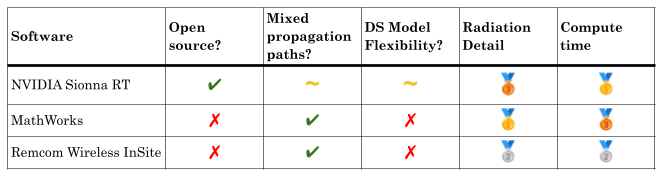
\includegraphics[width=3.5in]{RTSoftware}
\captionsetup{singlelinecheck=off}
	\caption[]{A comparison of some existing RT softwares (summarised from \cite{ref:RTComparison}). There's no clear winner, and a consistent lack of flexibility of implementation.}
\label{diag:RTSoftware}
\end{figure}

% TODO: Finish

\section{Conclusion}
From reviewing the literature, it's clear that modelling DS for RT in an outdoor setting is an active area of research with many exciting avenues. There are gaps in our existing models to accurately capture broad channel-dispersion characteristics like delay-spread, in addition to gaps in our modelling software.

Particularly,
\begin{enumerate}
	\item there's a need for more flexible RT software, and
	\item model / environmental simplifications in order to obtain channel information more rapidly.
\end{enumerate}

These two goals will be the focus of the research project.
% TODO: Finish

 % TODO: Properly format the References section, add in another reference,
\begin{thebibliography}{1}
\bibliographystyle{IEEEtran}

\bibitem{ref:degliSecond}
V. Degli-Esposti ``A diffuse scattering model for urban propagation prediction'', IEEE Transactions on Antennas and Propagation, vol. 49, no. 7, pp. 1111-1113, July 2001.

\bibitem{ref:degliThird}
V. Degli-Esposti, F. Fuschini, E. M. Vitucci and G. Falciasecca, ``Measurement and Modelling of Scattering From Buildings'', IEEE Transactions on Antennas and Propagation, vol. 55, no. 1, pp. 143-153, Jan. 2007.

\bibitem{ref:directiveRepl}
F. Mani and C. Oestges, ``Ray-tracing evaluation of diffuse scattering in an outdoor scenario'', Proceedings of the 5th European Conference on Antennas and Propagation (EUCAP), Rome, Italy, 2011.

\bibitem{ref:BK1}
Hossein Ragheb, Edwin R. Hancock, ``The modified Beckmann–Kirchhoff scattering theory for rough surface analysis'', Pattern Recognition, Volume 40, Issue 7, 2007, Pages 2004-2020, ISSN 0031-3203.

\bibitem{ref:BK2}
F. Sheikh, D. Lessy and T. Kaiser, ``A Novel Ray-Tracing Algorithm for Non-Specular Diffuse Scattered Rays at Terahertz Frequencies'', 2018 First International Workshop on Mobile Terahertz Systems (IWMTS), Duisburg, Germany, 2018, pp. 1-6.

\bibitem{ref:BK3}
F. Sheikh and T. Kaiser, ``A Modified Beckmann-Kirchhoff Scattering Model for Slightly Rough Surfaces at Terahertz Frequencies'', 2019 IEEE International Symposium on Antennas and Propagation and USNC-URSI Radio Science Meeting, Atlanta, GA, USA, 2019, pp. 2079-2080.

\bibitem{ref:reciprocalHeur}
E. M. Vitucci, N. Cenni, F. Fuschini and V. Degli-Esposti, ``A Reciprocal Heuristic Model for Diffuse Scattering From Walls and Surfaces'', IEEE Transactions on Antennas and Propagation, vol. 71, no. 7, pp. 6072-6083, July 2023.

\bibitem{ref:fieldPrediction}
V. Degli-Esposti, D. Guiducci, A. de'Marsi, P. Azzi and F. Fuschini, ``An advanced field prediction model including diffuse scattering'', IEEE Transactions on Antennas and Propagation, vol. 52, no. 7, pp. 1717-1728, July 2004.

\bibitem{ref:RTComparison}
M. Zhu, L. Cazzella, F. Linsalata, M. Magarini, M. Matteucci and U. Spagnolini, ``Toward Real-Time Digital Twins of EM Environments: Computational Benchmark for Ray Launching Software'', in IEEE Open Journal of the Communications Society, vol. 5, pp. 6291-6302, 2024.

\bibitem{ref:dynamicRTPaper}
Bilibashi, Denis & Vitucci, Enrico & Degli-Esposti, Vittorio, ``On Dynamic Ray Tracing and Anticipative Channel Prediction for Dynamic Environments''. IEEE Transactions on Antennas and Propagation. PP. 1-1. 10.1109/TAP.2023.3262155, 2023.

\end{thebibliography}

\end{document}
